\documentclass{article}
\usepackage{graphicx}
\usepackage{amsmath}
\usepackage{xcolor}
%\usepackage{biblatex}
%\addbibresource{citation-1.bib}

\title{ID2090 ASSIGNMENT: 4}
\author{ch22b118}
\date{}

\begin{document}
\maketitle
\section*{CH22B118:}
\begin{flushleft}
\textbf{Name: Sakshi Bapu Talapade}

\textbf{GitHub id: ch22b118}
\end{flushleft}

\section*{\begin{center}
    GAUSS'S LAW
\end{center}}

\subsection*{Introduction}

Gauss's law  ~\cite{inbook} is a fundamental principle in electromagnetism that relates the electric flux through a closed surface to the charge enclosed by that surface. It can be expressed in both integral and differential forms.


\subsection*{Integral Form}

The integral form of Gauss's law ~\cite{inbook} states that the electric flux $\Phi_E$ through a closed surface is equal to the total charge $Q$ enclosed by that surface divided by the permittivity of free space $\varepsilon_0$:

\textcolor{blue}{\[
\oint \mathbf{E} \cdot \mathrm{d}\mathbf{A} = \frac{Q}{\varepsilon_0}
\]}

where:
\begin{align*}
\oint & \text{ represents the surface integral over the closed surface}, \\
\mathbf{E} & \text{ is the electric field vector}, \\
\mathrm{d}\mathbf{A} & \text{ is the vector area element of the surface}, \\
Q & \text{ is the total charge enclosed by the surface}, \\
\varepsilon_0 & \text{ is the permittivity of free space}.
\end{align*}


\begin{figure}[h]
    \centering
    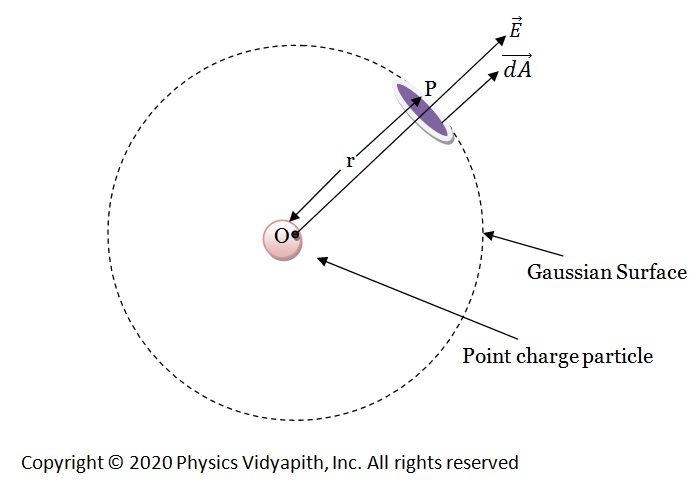
\includegraphics[width=10cm]{Electric Field Due to point charge particle_gauss law.jpg}
    \caption{Gauss's Law for a point charge}
    \label{fig:Gauss's Law}
\end{figure}

\subsection*{Differential Form}

The differential form of Gauss's law \cite{inbook} relates the divergence of the electric field $\mathbf{E}$ to the charge density $\rho$ within the volume enclosed by the surface:

\textcolor{blue}{\[
\nabla \cdot \mathbf{E} = \frac{\rho}{\varepsilon_0}
\]}

where:
\begin{align*}
\nabla & \text{ represents the divergence operator}, \\
\rho & \text{ is the charge density}, \\
\varepsilon_0 & \text{ is the permittivity of free space}.
\end{align*}

Gauss's law is a powerful tool for analyzing electric fields and charges, and it provides important insights into the behavior of electromagnetic systems.

\bibliography{citation-1}
\biibliographystyle{plain}

\end{document}
